%%%%%%%%%%%%%%%%%%%%%%%%%%%%%%%%%%%%%%%%%%%%%%%%%%
\begin{frame}{}
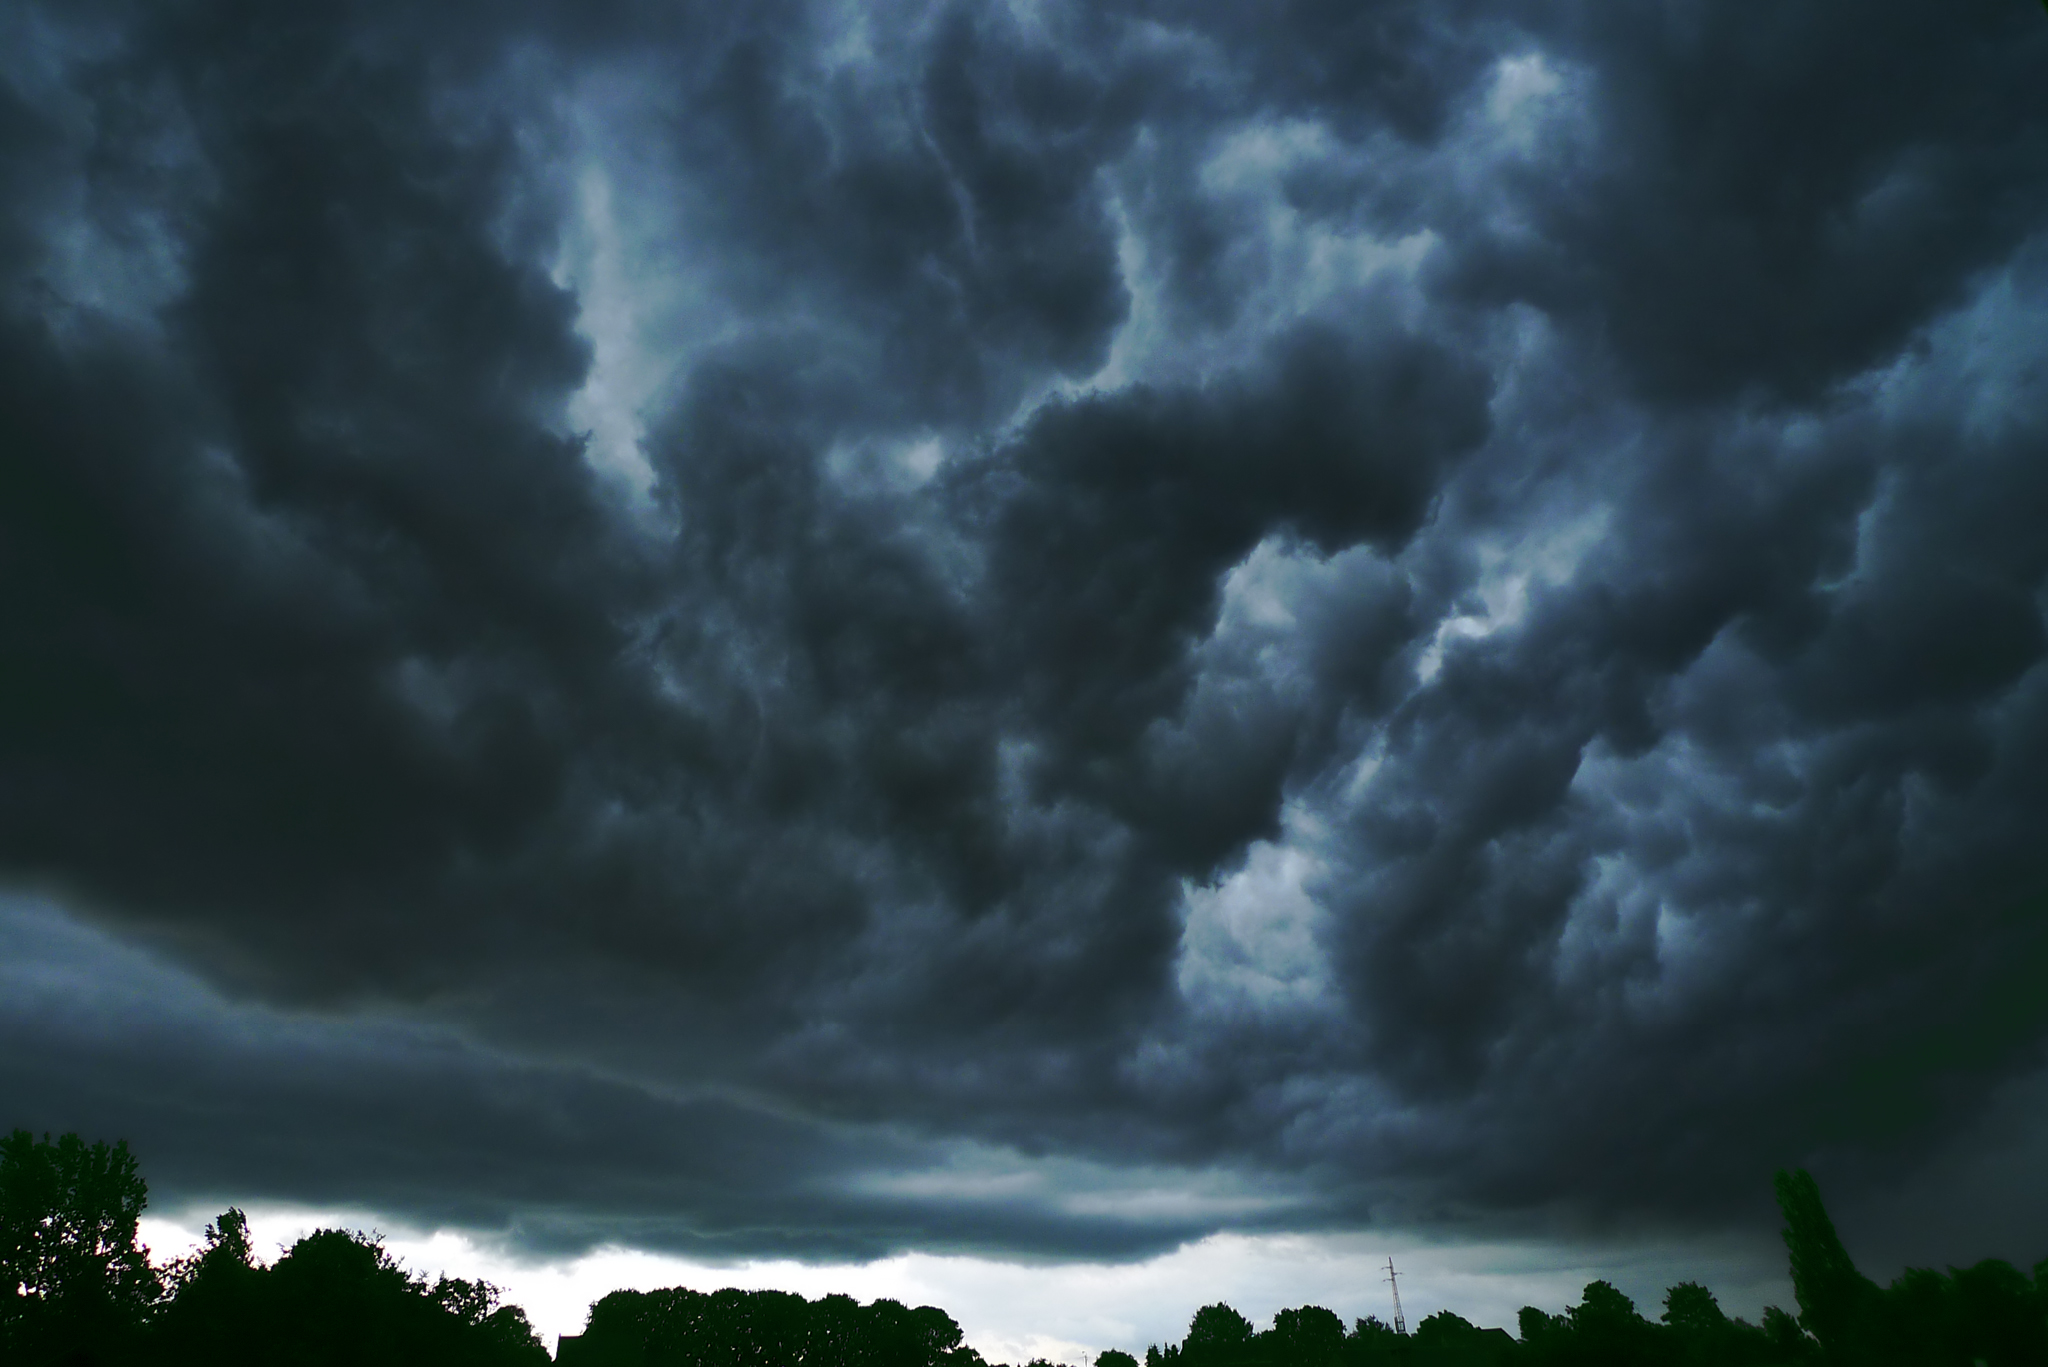
\includegraphics[width=\framewidth]{pics/thunderstorm.jpg}
% Copyright dimitri_c, http://www.freeimages.com/photo/1200003
% \paperwidth ??
\end{frame}

%%%%%%
\note{
\begin{description}
\item[N] Hallo
\item[J] Hi, na wie geht's?
\item[N] Uh, nicht so prima. Wir haben grad ziemlich viel Stress auf der Arbeit. Unsere neue Applikation wird kräftig entwickelt, aber irgendwie wird alles immer mühsamer... Guck mal hier:
\end{description}
}

%%%%%%%%%%%%%%%%%%%%%%%%%%%%%%%%%%%%%%%%%%%%%%%%%%
\begin{frame}{Unsere aktuelle Architektur}
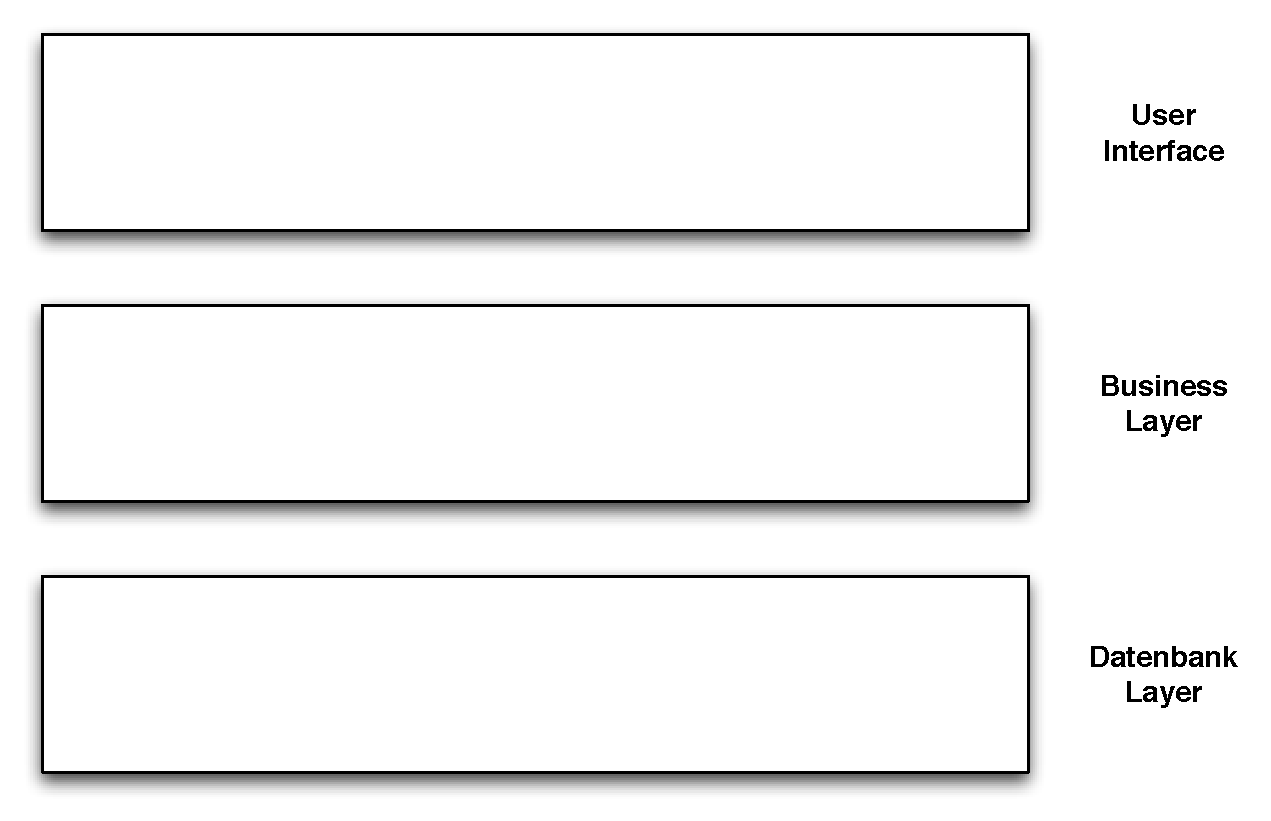
\includegraphics[width=\framewidth]{pics/Layer.pdf}

\end{frame}

%%%%%%
\note{
\begin{description}
\item[N] So sieht's gerade bei uns aus. Ganz normal, oder? UI-Layer, Business-Layer und Datenbank-Layer.
Aber irgendwie stellt sich heraus, dass unsere gesamte Logik total über die Schichten verschmiert ist. Guck mal hier:
\end{description}
}


%%%%%%%%%%%%%%%%%%%%%%%%%%%%%%%%%%%%%%%%%%%%%%%%%%
\begin{frame}{Unsere aktuelle Architektur}
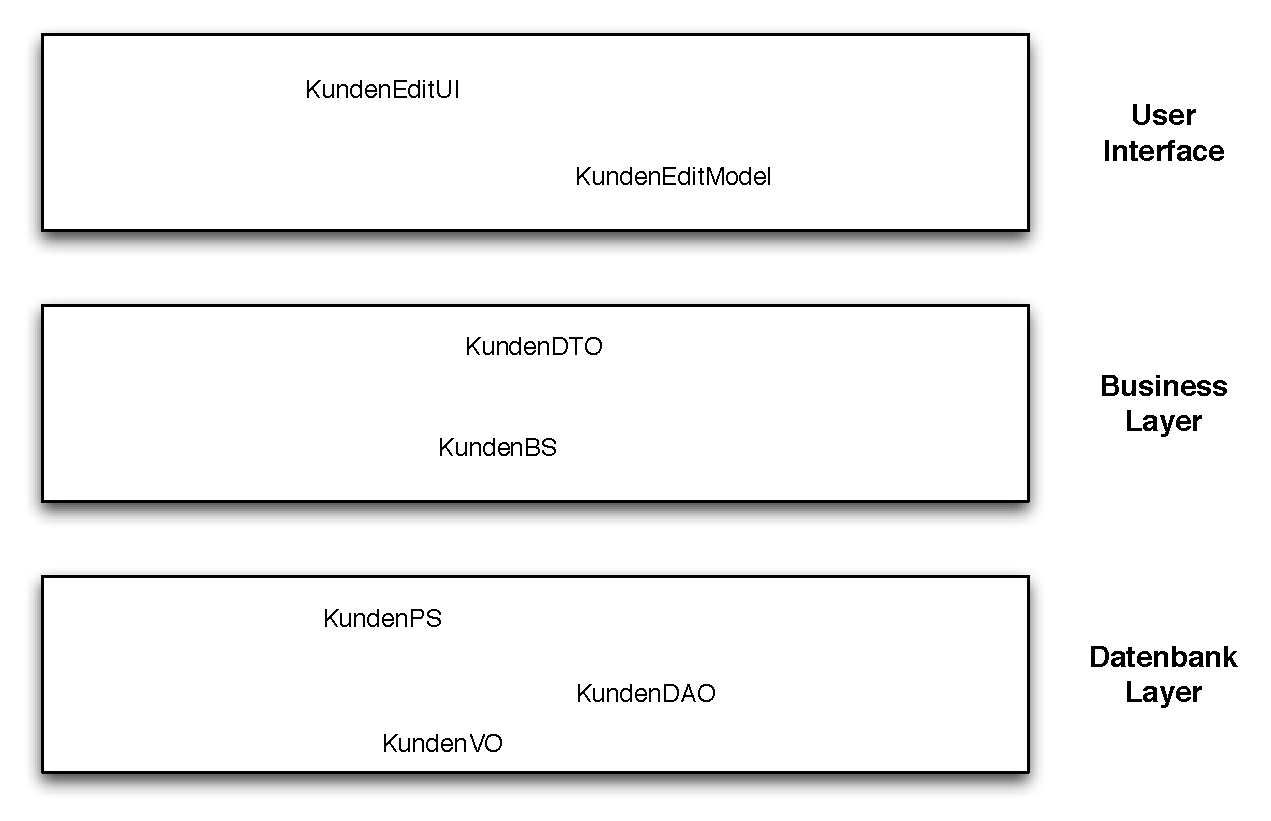
\includegraphics[width=\framewidth]{pics/LayerMitObjekten.pdf}
\end{frame}

%%%%%%
\note{
\begin{description}
\item[N] Schwierig, Tests zu schreiben / Technik auch / Auftraggeber versteht nur Bahnhof / wirft alle Abkürzungen durcheinander / alles ist aufgesplittert / Missverständnisse selbst bei Entwicklern / Jede Menge Impls und Managers
\item[J] Ja, das kenn ich gut. Wir waren auch mal in so einer Abkürzungs-Hölle.
\item[N] Waren? Das heißt, Ihr seid da rausgekommen? Und es gibt noch Hoffnung?
\item[J] Naja, geschenkt bekommen haben wir das natürlich auch nicht. Das war schon ganz schön Arbeit.
\item[N] Egal! Wie habt Ihr das gemacht, sag schon!
\end{description}
}
\note{
\begin{description}
\item[J] Naja, ... wir machen jetzt Domain-Driven Design.
\item[N] Hm, ich glaub davon hab ich schon gehört... DDD ... noch ne Abkürzung - nee, das hilft doch nicht weiter.
\item[J] Na, wart's mal ab, ich erzähl Dir einfach mal ein bisschen davon, ok?
\item[N] Na also gut... schlimmer kann's ja nicht mehr werden.
\end{description}
}

%%%%%%%%%%%%%%%%%%%%%%%%%%%%%%%%%%%%%%%%%%%%%%%%%%
\begin{frame}{Domain-Driven Design}
\begin{itemize}
\item versucht die Brücke zu schlagen zwischen Domänen-Experten und Entwicklern
\item fokussiert die Entwicklung auf die Fachlichkeit
\item gibt Entwicklern Bausteine und Werkzeuge in die Hand, um gute Anwendungen zu schreiben
\end{itemize}
\end{frame}

\begin{frame}{Oder so? Domain-Driven Design}
\begin{itemize}
\item Domänen-Experten und Entwickler gemeinsam
\item Fokus der Entwicklung auf die Fachlichkeit
\item Bausteine und Werkzeuge für gute Anwendungen
\end{itemize}
\end{frame}

%%%%%%
\note{
\begin{description}
\item[J] stellt die Punkte vor
\item[N] Das klingt ja sehr interessant! Aber ist das jetzt nicht wieder so ein neuer Hype?
\item[J] Nein - Teile schon Jahrzehnte alt
\item[J] DAS Buch ist über 10 Jahre alt
\item[N] OK. Aber bist Du wirklich sicher, dass das auch für uns passt?
\item[J] DDD ist besonders geeignet, wenn Fachlichkeit Kern der Anwendung / Abgegrenzte Domäne
\item[N] Das ist bei uns der Fall. Dann erzähl doch einfach mal weiter!
\end{description}
}

%%%%%%%%%%%%%%%%%%%%%%%%%%%%%%%%%%%%%%%%%%%%%%%%%%
\begin{frame}{Baustein: Entität}
\begin{itemize}
\item hat eine Identität (beschreibt das \glqq{}wer\grqq{})
\item hat einen Lebenszyklus
\item Modellierung fokussiert darauf
\item eindeutigen Identifikator festlegen
\end{itemize}
\end{frame}

%%%%%%
\note{
\begin{description}
\item[J] Identität gilt oft auch außerhalb der gerade betrachteten Software
\item[N] Ja, das kenne ich, wir modellieren Kunden, die haben natürlich auch im echten Leben einen Namen und ein Geburtsdatum
\item[J] Innerhalb des Lebenszyklus können sich Werte der Entität ändern
\item[N] Ja, das macht immer am meisten Stress, wenn die Kunden umziehen oder heiraten. Nicht so einfach, damit umzugehen...
\item[J] Genau, deswegen ist es wichtig, einen eindeutigen Identifikator festzulegen. Es könnten ja auch mal zwei Kunden denselben Namen haben.
\end{description}
}

\note{
\begin{description}
\item[N] Du meinst zum Beispiel die Objektidentität?
\item[J] Nein, da sollte man schon selbst etwas implementieren, Objektidentität passt meistens nicht genau. Insbesondere wenn man mit einer Datenbank arbeitet und immer wieder neue Instanzen einer Entität bekommt.
\item[N] Aber grundsätzlich ist es schon so, dass meine derzeitigen Datenbankobjekte alles Entitäten sind, oder? Dann verstehe ich noch nicht, was jetzt das Großartige und Neue sein soll...
\item[J] Nur Geduld! Ich vermute nämlich, dass nicht alle Deiner derzeitigen Datenbankobjekte Entitäten sind. Es gibt ja auch noch Value Objects.
\end{description}
}

%%%%%%%%%%%%%%%%%%%%%%%%%%%%%%%%%%%%%%%%%%%%%%%%%%
\begin{frame}{Baustein: Value Object}
\begin{itemize}
\item Wert
\item hat keine Identität (beschreibt \glqq{}was\grqq{}, nicht \glqq{}wer\grqq{})
\item Fachlicher Wrapper um technische Datentypen
\item bildet eine konzeptionelle Einheit
\item kann oft als Immutable implementiert werden
\begin{itemize}
\item dann ist Sharing möglich
\end{itemize}
\end{itemize}
\end{frame}

%%%%%%
\note{
\begin{description}
\item[J] Value Objects wendet man da an, wo man Werte repräsentieren will. Und wo die Identität keine Rolle spielt, also wo ich ein Value Objekt durch ein anderes identisches ersetzen kann.
\item[N] Also Du meinst Strings und ints und sowas?
\item[J] Im Prinzip schon. Aber die haben keine fachliche Semantik: Was bedeutet dieser Double, welche Werte sind hier gültig?
\item[N] Oh ja, das kenne ich. Wir haben eine Methode mit 10 Parametern, alles Doubles. Der häufigste Bug an der Stelle ist, dass irgendjemand mal wieder die Werte in der falschen Reihenfolge übergeben hat...
\end{description}
}
\note{
\begin{description}
\item[J] Und deswegen ist es sinnvoll, fachliche Wrapper-Klassen zu erstellen, die die Semantik ausdrücken. Simple Beispiele sind Geldbetrag oder Prozentsatz.
Interessant dabei ist, dass man Value Objects oft als immutable implementieren kann, d.~h.~dass man das Objekt nach der Erzeugung nicht mehr verändern kann.
\item[N] Hm, aber was ist, wenn sich jetzt was ändert, zum Beispiel die Gesamtsumme in meinem Warenkorb?
\end{description}
}

\note{
\begin{description}
\item[J] Da kann ich einfach einen neuen Geldbetrag mit der neuen Gesamtsumme bauen und den alten dadurch ersetzen. Und die Implementierung meines Value Objects wird dadurch viel einfacher. Man kann sogar häufig vorkommende Value Objects wiederverwenden - das ist ungefährlich, denn sie können ja nicht verändert werden.
\item[N] Ah, klingt interessant! Wir haben ganz oft einen Preis von 99 Cent, da könnte ich dann immer dasselbe Value Object verwenden, oder?
\item[J] Ja, zum Beispiel.

\item[N] Mensch, danke für die vielen Infos! Jetzt bin ich mal gespannt, wie wir das Ganze bei uns im Team umsetzen können. Tschüs, ich muss los!
\end{description}
Gehen ab.
}

%%%%%%%%%%%%%%%%%%%%%%%%%%%%%%%%%%%%%%%%%%%%%%%%%%
\begin{frame}{Einige Wochen später...}

\includegraphics[width=\framewidth]{pics/dandelions.jpg}
% Copyright Krappweis, http://www.freeimages.com/photo/1429166
\end{frame}

%%%%%%
\note{
\begin{description}
\item[J] Hallo, schön Dich wiederzusehen! Wie läuft's denn so mit Domain-Driven Design?
\item[N] Oh, sehr gut! Wir haben inzwischen einige unserer Probleme in den Griff bekommen und auch coole neue Sachen entdeckt.
\item[J] Das ist ja schön zu hören! Magst Du mir was davon erzählen?
\end{description}
}

%%%%%%%%%%%%%%%%%%%%%%%%%%%%%%%%%%%%%%%%%%%%%%%%%%
\begin{frame}{Neues über Value Objects}
\begin{itemize}
\item aus Entitäten auslagern
\item können auch komplexer aufgebaut sein
\item entwickeln sich zu \glqq{}Code-Magneten\grqq{}
\end{itemize}
\end{frame}

%%%%%%
\note{
\begin{description}
\item[N] wir hatten ziemlich viele riesige Entitäten, z. B. hat unser Kunde alle Angaben über ihn direkt als Attribute gehabt: Alle Namens- und Adressbestandteile, Telefonnummer, Kreditkartennummer und was noch alles. Davon haben wir den Großteil herausgezogen und in spezialisierten Value Objects untergebracht. Der Kunde kennt jetzt nur noch diese Value Objects und nicht mehr die Details.
\item[N] Ein interessanter Nebeneffekt: Wir machen jetzt auch komplexe Value Objects, nicht nur simple Wrapper. Wie zum Beispiel unsere Adresse.
\end{description}
}

\note{
\begin{description}
\item[J] Eine Adresse ist ein gutes Beispiel für ein komplexes Value Object in der Domäne \glqq{}Online-Store\grqq{}. Denk nur dran, dass es in anderen Domänen ganz anders sein kann. In einer Grundstücksverwaltung oder in einer Briefzustellungssoftware wird man Adressen vermutlich eher als Entitäten modellieren. 
\item[N] Hm...
\item[J] Aber ich hab Dich unterbrochen. Was hast Du denn sonst noch so rausgefunden?
\end{description}
}

\note{
\begin{description}
\item[N] Das coolste ist: Die Value Objects ziehen den Code förmlich an! Alles, was mit einem Value Object zu tun hat, implementieren wir dort als Methode: z. B. Validierung oder das Herausziehen von Teilaspekten (... ?!)
Früher war dieser Code im ganzen System verstreut, und meistens hat man ihn nicht wiedergefunden, wenn man ihn gebraucht hat, und hat alles nochmal implementiert, und nochmal... Jetzt gibt es einen klaren Platz für diesen Code, das ist super!
\item[J] Mir scheint, Ihr seid auf einem richtig guten Weg!
\item[N] Aber es knirscht auch noch ganz schön an vielen Stellen.
\end{description}
}

\note{
\begin{description}
\item[J] Wo denn zum Beispiel?
\item[N] Naja, wir Entwickler kommen noch nicht so gut klar mit den Leuten vom Fachbereich. Sie sprechen eine ganz andere Sprache als wir, zum Beispiel sagen sie "Artikel", und das heißt bei uns im Code "Bestellposition". Einer von uns hat das gut im Griff und spielt immer den Übersetzer. Aber wenn der nicht da ist, läuft echt gar nix. Manchmal benutzen aber auch alle denselben Begriff, meinen nur etwas komplett Unterschiedliches. Dass hinterher nix zusammenpasst, ist da ja fast schon garantiert.
\item[J] Dass eine gemeinsame Sprache sehr wichtig ist, das ist auch ein Schwerpunkt von DDD.
\end{description}
}



%%%%%%%%%%%%%%%%%%%%%%%%%%%%%%%%%%%%%%%%%%%%%%%%%%
\begin{frame}{Die allgegenwärtige und gemeinsame Sprache}
\begin{itemize}
\item Fachbegriffe überall verwenden, auch im Code!
\item Glossar zur Begriffsklärung
\item Muss reichhaltig genug sein  für sämtliche Kommunikation
\item Beschreibt nicht nur die Einheiten im System, sondern auch Aufgaben und Funktionalitäten
\item Muss widerspruchsfrei und eindeutig sein
\end{itemize}
\end{frame}

%%%%%%
\note{
\begin{description}
\item[J] Du hast ja selbst schon festgestellt, wie wichtig und schwierig die Sprache ist. Alle müssen dieselbe Sprache sprechen - vom Auftraggeber über den Fachbereich bis zum Entwickler. Idealerweise solltest Du dem Auftraggeber den Namen irgendeiner Klasse nennen können, und er kann sich etwas darunter vorstellen.
\item[N] Hm, also das klappt bei uns noch nicht so gut, bei unserem KundeVO kann sich unser Auftraggeber echt nichts vorstellen, komisch eigentlich.
\item[J] Naja, ein VO gibt es in seiner Fachlichkeit nun mal nicht. Hast Du vielleicht einen besseren Namen für die Klasse?
\end{description}
}

\note{
\begin{description}
\item[N] Naja, eigentlich ist es ja ein Kunde - also wie wäre es damit? Ginge das? Einfach nur "Kunde"?
\item[J] Klar, das wäre ziemlich gut.
\item[N] Aber das ist ja sicher noch nicht alles.
\item[J] Das Wichtigste hierbei ist sicherlich, konsequent zu sein. Die gemeinsame Sprache muss alles umfassen und muss in allen Gesprächen benutzt werden - egal ob da nur Entwickler oder nur Fachler oder beide miteinander reden. Ein Glossar hilft ungemein, um die Begriffe zu schärfen, damit es möglichst wenige Missverständnisse gibt. Und natürlich darf jeder Begriff nur für genau eins verwendet werden - wenn's mehrdeutig wird, muss man gemeinsam überlegen, wie man das auflösen kann.
\end{description}
}

\note{
\begin{description}
\item[N] Und wenn ich mal merke, dass ich einen ungeschickten Begriff eingeführt habe, und den ändern möchte? Dann muss ich vermutlich auch in meinem Code alles umbenennen, oder?
\item[J] Ja genau. Ich sehe, so langsam findest Du Zugang zu dem Thema :-)
\end{description}
}


%%%%%%%%%%%%%%%%%%%%%%%%%%%%%%%%%%%%%%%%%%%%%%%%%%
\begin{frame}{Domain Services}
\begin{itemize}
\item TODOOOO
\end{itemize}
\end{frame}

%%%%%%
\note{
\begin{description}
\item[N] x
\item[J] x
\end{description}
}


%%%%%%%%%%%%%%%%%%%%%%%%%%%%%%%%%%%%%%%%%%%%%%%%%%
\begin{frame}{Repositories}
\begin{itemize}
\item Fachliche Schnittstelle zu Daten
\item Gaukeln In-Memory-Collection vor
\item Keine Infrastruktur-Abhängigkeiten in Domain Code
\end{itemize}
\end{frame}

%%%%%%
\note{
\begin{description}
\item[N] Gut, dass ich Dich treffe. Ich bin da nämlich gestern auf ein Design-Problem gestoßen, bei dem mir ein wenig der Durchblick fehlt.
\item[J] Dann schieß mal los. Vielleicht kann ich ja helfen.
\item[N] Wir hatten bisher vor allem die Kern-Fachlichkeit im Blick. Value Objects, Entities und Services haben wir das recht gut abbilden können. Jetzt wollten wir aber mal eine Datenbank anbinden. Ich habe da mal die Bücher gewälzt und bin über Repositories gestoßen.
\item[J] Genau - gut, dass  Du das gefunden hast.
\end{description}
}

\note{
\begin{description}
\item[N] Wir sind da mal ganz nach Lehrbuch drangegangen und haben uns eine Schnittstelle gebaut, bei der wir einfach nur fachlich beschreiben, welche Daten wir lesen, löschen oder speichern wollen. Von der Ansteuerung ist das dann in etwa so, als ob es eine Collection wäre, die im Speicher liegt. Nur dass ich fachliche Zugriffsmethoden habe. Technische Klassen werden in der Schnittstelle nicht referenziert, also nichts aus Persistence-Frameworks oder ähnlichem.
\item[J] Das klingt doch schon mal sehr vernünftig. Verstehe ich das richtig, dass Ihr eine Trennung von Schnittstelle und Implementierung habt?
\end{description}
}

\note{
\begin{description}
\item[N] Ja genau. Wir haben die Schnittstelle, also z.B. das KundenRepository. Irgendwo muss dann natürlich auch mal wirklich eine Datenbank angesprochen werden. Das passiert dann in der Klasse KundenDatabaseRepository. Dort werden dann Queries gebaut oder der OR-Mapper angeworfen. In unseren Domain-Services, wo wir die Repositories verwenden, sind wir dann aber absolut Datenbank-los unterwegs.
\item[J] Und wo ist Euer Problem?
\item[N] Wie strukturieren wir das am Besten? Ich zeige es Dir mal kurz im Diagramm, was ich meine:
\end{description}
}


%%%%%%%%%%%%%%%%%%%%%%%%%%%%%%%%%%%%%%%%%%%%%%%%%%
\begin{frame}{Repositories}
\begin{itemize}
\item TODOOOOO: Bild mit klassischer Schichtung
\end{itemize}
\end{frame}

%%%%%%
\note{
\begin{description}
\item[N] Wir haben wir unseren Domain Service. Der programmiert sauber gegen die Schnittstelle des Repositories, sobald ich aber dann doch die wirkliche Implementierung für die DB verwenden will, habe ich doch die Abhängigkeit aus der Domain zur Datenbank, also zu technischen Dingen. Das will ich so doch nicht haben, oder? 
\item[J] Das ist wirklich nicht so ideal. Natürlich bist Du schonmal deutlich besser unterwegs als davor! Du hast alle Fachlichkeit in einer Schicht angesiedelt. Aber diese Abhängigkeit fühlt sich irgendwie falsch an.
\end{description}
}

\note{
\begin{description}
\item[N] Letzten Endes habe ich aber keine andere Option, wenn ich mich an die Schichtenarchitektur halten will. Alle Zugriffe müssen ja von oben nach unten gehen. Von unten nach oben ist verboten.
\item[J] Stimmt, das klassische 3-Tier-Schichten-Modell mit UI - Business - Persistence führt zu diesem Phänomen. Es gibt aber auch noch eine andere Art, wie man das ganze betrachten kann. Die finde ich inzwischen einleuchtender. Halte Dich mal gut fest, beim ersten Betrachten kann es einem da schon mal kurz schwindlig werden.
\end{description}
}


%%%%%%%%%%%%%%%%%%%%%%%%%%%%%%%%%%%%%%%%%%%%%%%%%%
\begin{frame}{Repositories}
\begin{itemize}
\item TODOOOOO: Bild mit Innen-Außen-Architektur.
\end{itemize}
\end{frame}

%%%%%%
\note{
\begin{description}
\item[N] Uuuups - wie muss ich das jetzt verstehen?
\item[J] Wenn wir die Architektur so darstellen, dass stellen wir die Domäne ins Zentrum. 
\item[N] Das passt ja auch zu unserer ganzen Vorgehensweise bisher. Die Fachlichkeit ist das Kernstück der Software.
\item[J] Statt von oben und unten reden wir eher von innen und außen. Innen ist also die Domäne. Außen ist der Rest der Welt, mit dem wir in Verbindung stehen. Wir können über verschiedene Kanäle Nachrichten nach außen loswerden oder auch von außen angestoßen werden. Wir definieren eine fachliche Schnittstelle innen. Die Anbindung nach außen passiert dann über einen Adapter. Die Implementierung des Repositories ist dann so ein Adapter. 
\end{description}
}

\note{
\begin{description}
\item[J] Dort wird die Schnittstelle z.B. auf eine SQL oder NO-SQL-DB adaptiert.
\item[N] Und wo kriege ich einen solchen Adapter dann her? Auf Deinem Bild hier sieht es ja so aus, als ob es keine Zugriffe aus  der Domäne auf die Außenwelt gibt.
\item[J] Gut erkannt! Dort wo ich ein Repository brauche - also typsicherweise in einem Domain Service, wünsche ich mir einfach ein Repository - also erwarte das z.B. als Konstruktor-Argument. Das Wiring mit der Datenbank-Implementierung erfolgt dann durch das Zusammenbauen der Anwendung. Dependency Injection ist das Stichwort.
\item[N] Ach so - Du meinst Spring oder CDI!
\end{description}
}

\note{
\begin{description}
\item[J] Nicht unbedingt. Klar - ich kann mir das Zusammenbauen von einem Container oder Framework abnehmen lassen. Oft ist das auch eine gute Idee. In einfachen Fällen kann ich aber auch einfach in der main-Methoden die richtigen Implementierungen instanziieren und dann miteinander verheiraten.
\item[N] Moment mal - ich glaub, jetzt sehe ich wo das hinführt. Das hilft mir auch beim Testen. Auch hier baue ich mir ja einen Teil der Anwendung zusammen. Da habe ich die Wahl, ob ich ein "echtes" also DB-gebundenes Repository verwende, oder einfach nur einen Mock oder Stub, der die Daten in einer Collection hält. Das ist wirklich elegant. Ich habe gesehen, hier gibt es noch andere Adapter. Wozu sind die da?
\end{description}
}

\note{
\begin{description}
\item[J] Bisher haben wir ja vor allem über Repositories geredet, also, wo die Daten herkommen oder hingehen. Die anderen Adapter beschreiben vor allem die Wege in die Domäne. Also, wie werden fachliche Prozesse getriggert. Wie sieht die Anbindung aus. Auch hier sind ja die unterschiedlichsten Wege denkbar: GUI, REST-/SOAP-Schnittstelle, ... Rein technisch sehen die entsprechenden Ansteuerungsstrecken ja oft extrem unterschiedlich aus. Letzten Endes ist die fachliche Schnittstelle, bei der sie landen ja immer die gleiche. Ob ich jetzt einen "Bestellen"-Knopf drücke oder per Rest-Call das Signal dazu gebe, letzten Endes soll ja das gleiche passieren.
\end{description}
}

\note{
\begin{description}
\item[N] Und auch das ist ja für das Testen wieder geschickt. Ich kann mir einen Testtreiber schreiben, der einfach auf der Domänenschicht aufsetzt. Das ist ja auch nur ein weiterer Adapter.
\item[J] Ganz genau. Wenn ich mein System so strukturiere, dann stelle ich die Domäne ins Zentrum. Die Interaktion mit außen geschieht über Ports und Adapters. Das zwingt mich dazu, dass ich mir über meine Schnittstelle sehr bewusst bin. Aber das ist ja immer ein gute Idee. In einem ersten Schritt setze ich dann vielleicht einen Rest-Adapter drauf. Wenn dann später die Anforderungen sich ändern und ich eine SOAP-Schnittstelle brauche, weil ein Kunde das nur so bei sich integrieren kann, dann brauche ich nur einen weiteren Adapter. Der ist dann nochmal zu testen.
\end{description}
}

\note{
\begin{description}
\item[J] Innendrin ändert sich aber erstmal gar nichts.
\item[N] Nochmal zu meiner Frage mit den Repositories und der Strukturierung...
\item[J] Stimmt, da  waren wir ja gestartet. In der Domäne definierst Du Deine gewünschte Schnittstelle. Die Implementierung kann dann in separaten Packages oder sogar in einem eigenen Modul  erfolgen. Natürlich muss die Implementierung ihre Schnittstelle kennen. In die andere Richtung ist aber keine Abhängigkeit notwendig.
\item[N] Okay - das  macht Sinn. Da muss ich jetzt mal ein paar Sachen umbauen gehen. Danke auf jeden Fall fürs Erklären.
\end{description}
}


%%%%%%%%%%%%%%%%%%%%%%%%%%%%%%%%%%%%%%%%%%%%%%%%%%
\begin{frame}{Einige Monate später...}

\includegraphics[width=\framewidth]{pics/dandelions.jpg}
% Copyright Krappweis, http://www.freeimages.com/photo/1429166
\end{frame}

%%%%%%
\note{
\begin{description}
\item[N] Dass ist ja schön, dass wir uns mal wieder sehen!
\item[J] Freut mich auch. Erzähl doch mal, wie es bei Euch jetzt inzwischen so läuft? Kommt Ihr gut voran?
\item[N] Oh ja - wir sind sehr zufrieden. Natürlich klappt nicht alles perfekt. Aber gerade gestern hatte ich mal wieder so ein Aha-Erlebnis. Wir hatten beim Sprint-Review bemerkt, dass wir bei der Rabattberechnung einen Randfall nicht richtig umgesetzt hatten. Ich habe direkt danach kurz in den Code geschaut. Und mein Fachler saß noch da und hat auf einmal angefangen, mit mir im Code zu lesen. Der Hammer war, dass er den Fehler vor mir gefunden hat. Dadurch, dass er die Begriffe im Code kannte, haben ihn die ganzen eckigen und geschweiften Klammern anscheinend nicht gestört.
\end{description}
}

\note{
\begin{description}
\item[J] Das klingt ja echt, als ob alles in eine gute Richtung geht.
\item[N] Das denke ich auch. Wir merken jetzt einfach, dass es sich ausgezahlt hat, in ein passendes Objekt-Modell zu investieren. Das steht jetzt einfach bombensicher.
\item[J] Ähhmmm. Da wäre ich mir mal nicht zu sicher.
\item[N] Wieso - alle Funktionalität und Logik ist dort, wo sie hingehört.
\item[J] Es kann theoretisch schon sein, dass das jetzt so bleibt, aber das ist nicht so wahrscheinlich. Das kann verschiedene Gründe haben.
\item[N] Und welche könnten das sein?
\end{description}
}


%%%%%%%%%%%%%%%%%%%%%%%%%%%%%%%%%%%%%%%%%%%%%%%%%%
\begin{frame}{Gründe für Anpassungen am Modell}
\begin{itemize}
\item Grund Nummer 1: Lernen
\item Bessere Begriffe
\item Beziehungen werden klarer
\item Neue Konzepte/Abstraktionen tauchen auf
\end{itemize}
\end{frame}

%%%%%%
\note{
\begin{description}
\item[J] Meistens hängt es damit zusammen, dass man im Laufe der Zeit lernt. 
\item[N] Das ist klar. am Anfang muss man irgendwann mal loslegen, sonst bleibt man ewig in der Analyse stecken und man bekommt nie ein System, das irgendwas tut.
\item[J] Gleichzeitig ist es halt so, dass man zu Beginn am wenigsten Informationen und Erfahrung hat. Daher besteht schon die Gefahr, dass man Entscheidungen trifft, die nicht auf Dauer tragen. Im einfachsten Fall kann das sein, dass man einen Begriff wählt, der letztendlich doch nicht der ideale war.
\item[N] Und was macht man dann? Man kann ja nicht ständig alles umbenennen. Es hilft ja nicht, dass man im Glossar einen Eintrag ändert. 
\end{description}
}

\note{
\begin{description}
\item[N] Das zieht sich ja durch alles durch: Akzeptanztests, Code im schlimmsten Fall sogar Datenbank-Tabellen.
\item[J] Im besten Fall kommt das ja nicht sooo oft vor, dass man sich vergriffen hat. Aber Du hast schon recht: Das zieht sich dann durch. Durch einfache Text-Suche und Ersetzen erwischt man dann aber doch das meiste, wenn der Begriff davor einheitlich verwendet wurde. Wenn bei uns der Verdacht aufkommt, dass wir einen Begriff ersetzen sollten, dann nehmen wir den erstmal auf eine Liste auf und beobachten das ein wenig für uns. Die eigentliche Ersetzung ziehen wir dann mal möglichst schnell durch, wenn es ein wenig ruhiger ist. Dann haben wir nicht ganz so viel zu Mergen. Oft sind es aber auch etwas harmlosere Änderungen am Modell, die sich nicht so sehr durchziehen.
\end{description}
}

\note{
\begin{description}
\item[N] Zum Beispiel?
\item[J] Oft merkt man, dass die Art der Beziehungen zwischen zwei Klassen nicht geschickt gewählt wurde. In manchen Teams ist der Reflex, dass fast alle Assoziationen bi-direktional umgesetzt werden, damit man ja von jedem Objekt aus den gesamten Graph durchlaufen kann. Das führt dann zu unnötigen Zyklen. Meistens ist die Richtung, in die ich laufe, von der Fachlogik recht klar vorgegeben. Wenn man dann merkt, dass eine Richtung nicht oder nicht mehr nötig ist, dann sollte man die dringend rausmachen. Denn das vereinfacht das Modell, was eigentlich immer gut ist. 
\end{description}
}

\note{
\begin{description}
\item[N] Aber manchmal geht's auch in die andere Richtung: Im letzten Sprint ...: Das sind wir mit einer uni-direktionalen Beziehung gestartet und haben dann später gemerkt, dass das nicht reichte.
\item[J] Wichtig ist immer, dass die Software soft bleibt. Das Modell soll möglichst geschmeidig bleiben, damit wir weiter modellieren können. Und nichts ist für die Änderbarkeit besser, als wenn man häufig Änderungen vornimmt.
\item[N] Wahrscheinlich ist das dann auch die Argumentation, mit der ich das verkauft kriege, wenn ich schon wieder am Refactoren bin. Jeder in der Firma sollte ja ein Interesse daran haben, dass die Software nicht irgendwann total starr und unflexibel wird.
\end{description}
}

\note{
\begin{description}
\item[J] Das stimmt. Wo Du gerade das Stichwort Refactoring verwendest: Manchmal genügen die klassischen Refactorings - wie die von Martin Fowler - hier nicht. 
\item[N] Wie meinst Du das?
\item[J] Die meisten der klassischen Refactorings setzen eher darauf, dass man kleinere Schritte macht. So etwas wie das Umbenennen, von dem wir gerade schon sprachen. Es kommt aber auch immer wieder vor, dass man merkt, dass ein komplettes Konzept geändert werden muss.
\item[N] Woran kann ich das merken?
\item[J] Ein klassisches Symptom ist, dass ständig Begriffe verwendet werden, die sich nicht im Glossar wiederfinden 
\end{description}
}

\note{
\begin{description}
\item[J] und irgendwie so zwischen den Stühlen sind. Wenn das immer wieder auftaucht, dann will ich das auch im Code wiederfinden. Sobald ich im Kopf ein Mapping vornehmen oder jemanden fragen muss, wo etwas implementiert ist, bin ich wahrscheinlich schon in Schwierigkeiten. Ein anderer Bereich sind Validierungen und Constraints.
\item[N] Ich hatte gedacht, dass wir das immer direkt an den Objekten machen. Bei den Value Objects im Normalfall direkt bei der Erzeugung. Oft ist der Code zuerst mitten in einer Methode. Dann ziehen wir das aber immer in eine private Methode, die einen Namen bekommt, der die Fachlichkeit widerspiegelt. Damit fahren wir auch ganz gut bisher.
\end{description}
}

\note{
\begin{description}
\item[J] Das ist oft auch genau das richtige. Es kann aber auch sein, dass die Art der Validierung je nach Kontext unterschiedlich sein kann. Wenn dann das Objekt unterschiedlichste Fälle unterscheiden muss, führt das bald zur Überfrachtung mit Logik. Typischerweise ändern sich die Validierungen auch unabhängig vom Rest eines Objekts. Da kann dann eine Validierungs-Regel als Strategieklasse der bessere Weg sein, das zu modellieren.
\item[N] Klingt sinnvoll. Je nach Kontext kann ich die entsprechende Strategie verwenden. Die einzelnen Strategien kann ich dann unabhängig ändern und auch isoliert testen, während das Kernobjekt nicht zu sehr aufgebläht wird.
\end{description}
}

\note{
\begin{description}
\item[J] TODO!!!!!!!!!!!!!!!!: Salbungsvolle Überleitung
\end{description}
}


% FAZIT:
%%%%%%%%%%%%%%%%%%%%%%%%%%%%%%%%%%%%%%%%%%%%%%%%%%
\begin{frame}{Achtung!}
\begin{itemize}
\item Technisches nicht hinten runterfallen lassen
\item Vorsicht vor blutleeren Modellen - Code in die Objekte!
\end{itemize}
\end{frame}

%%%%%%
\note{
\begin{description}
\item[N] x
\item[J] x
\end{description}
}


%%%%%%%%%%%%%%%%%%%%%%%%%%%%%%%%%%%%%%%%%%%%%%%%%%
\begin{frame}{Was man beherzigen darf}
\begin{itemize}
\item Gutes Zusammenspiel mit Specification by Example bzw. ATDD
\end{itemize}
\end{frame}

%%%%%%
\note{
\begin{description}
\item[N] x
\item[J] x
\end{description}
}



% TEMPLATE:
%%%%%%%%%%%%%%%%%%%%%%%%%%%%%%%%%%%%%%%%%%%%%%%%%%
\begin{frame}{x}
\begin{itemize}
\item x
\end{itemize}
\end{frame}

%%%%%%
\note{
\begin{description}
\item[N] x
\item[J] x
\end{description}
}


%%%%%%%%%%%%%%%%%%%%%%%%%%%%%%%%%%%%%%%%%%%%%%%%%%
{
\usebackgroundtemplate{
\includegraphics[width=\paperwidth,height=\paperheight]{background-slide.png}}
\begin{frame}{Vielen Dank!}

        Folien auf GitHub:
        \vspace{-0.8em}
        \begin{center}
                \url{https://github.com/NicoleRauch/DomainDrivenDesign}
        \end{center}

        \begin{block}{Jens Borrmann}
        \begin{description}[Twitterxx]
                \item[E-Mail]  \href{mailto:jens.borrmann@msg-gillardon.de}{\texttt{jens.borrmann@msg-gillardon.de}}
                \item[Twitter] \href{http://twitter.com/jborrmann}{\texttt{@jborrmann}}
        \end{description}
        \end{block}
        \begin{block}{Nicole Rauch}
        \begin{description}[Twitterxx]
                \item[E-Mail]  \href{mailto:nicole.rauch@msg-gillardon.de}{\texttt{nicole.rauch@msg-gillardon.de}}
                \item[Twitter] \href{http://twitter.com/NicoleRauch}{\texttt{@NicoleRauch}}
        \end{description}
        \end{block}
\end{frame}
}
